\scanpage{117}
\mspage{3}

Les notations introduites sont telles qu'elles gardent un sens pour toute carte triangulaire ``polarisée'' de type $\{0,1,\infty\}$, sans que celle\deleted{\unsure{soit la|qui est la}} \inserted{-ci soit} nécessairement : la subdivision barycentrique d'une carte $X$, condition qui s'exprime par la 
\begin{tikzpicture}[baseline=(condition117.base)]
\node[anchor=base west,inner sep=0pt] (condition117) at (0,0) {\deleted{condition}};
\node[anchor=south west,inner sep=0pt] (derniere117)
  at ([xshift=-4pt,yshift=4pt]condition117.north west) {\inserted{dernière}};
\draw[line width=.35pt] ([xshift=-4pt,yshift=-2pt]condition117.west)
  .. controls ([xshift=-4pt,yshift=4pt]condition117.north west)
  and ([xshift=-1pt,yshift=-1pt]derniere117.south west) .. (derniere117.south west)
  -- ([xshift=-1pt,yshift=-1pt]derniere117.south east)
  .. controls ([xshift=2pt,yshift=-1pt]derniere117.south east)
  and ([xshift=3pt,yshift=0pt]derniere117.south east)
  .. ([xshift=2pt,yshift=2pt]derniere117.south east);
\end{tikzpicture} relation
\[
\deleted{\unsure{\tau_0\tau_\infty|\tau_0}}\qquad (\tau_0\tau_\infty)^2=1\qquad\text{i.e}\quad\rho_1^2=1
\]
dans $(4)$ (qu'on abandonne donc par la suite) et qui signifie aussi que les \deleted{points} \inserted{sommets} de type $1$ sont d'ordre réduit $2$ (d'ordre ordinaire $4$), ou encore que $\tau_0\tau_\infty(r)=\tau_\infty\tau_0(r)$ pour tout $r$. Dans le cas général, $\rho_1$ est donc une op. qui ne joue plus un rôle particulier p.r. à $\rho_0,\rho_\infty$ : c'est la rotation ``d'un cran'' de $r$ autour du sommet de type $1$, dans le \deleted{\unsure{demi-tour} \unsure{indiqué|défini}} \inserted{sens défini} par l'orientation de $r$.

On introduit
\[
(13)\qquad\left\{
\begin{aligned}
\Lambda_r^i&=(\lambda_{\tau_{i+1}}^i)^{-1}\lambda_r^i:R_r^{i,i+1}\mathrel{\tikz[baseline=-.5ex]{\draw[line width=.45pt] (0,0)--(.6,0)--(.6,.07);}} R_{\tau_{i+1}(r)}^{i,i+1}\\
\Lambda_r^{\prime i}&=\lambda_{\sigma_{i-1}(r)}^i(\lambda_r^i)^{-1}:R_r^{i,i-1}\mathrel{\tikz[baseline=-.5ex]{\draw[line width=.45pt] (0,0)--(.6,0)--(.6,.07);}} R_{\tau_{i-1}(r)}^{i-1}
\end{aligned}\right.
\]
rotation d'un double cran'' autour du sommet de type $i$ de $r$, à partir du sommet proche de type 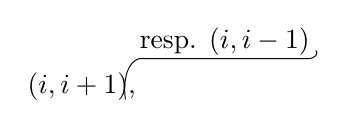
\begin{tikzpicture}[baseline=(type117.base)]
\node[anchor=base west,inner sep=0pt] (type117) at (0,0) {$(i,i+1)$,};
\node[anchor=south west,inner sep=0pt] (resptype117)
  at ([xshift=1pt,yshift=6pt]type117.north east) {\inserted{resp. $(i,i-1)$}};
\draw[line width=.35pt] ([xshift=-4pt,yshift=-2pt]type117.base east)
  .. controls ([xshift=-5pt,yshift=3pt]type117.east)
  and ([xshift=-4pt,yshift=-2pt]resptype117.south west)
  .. ([xshift=0pt,yshift=-1pt]resptype117.south west)
  -- ([xshift=-1pt,yshift=-1pt]resptype117.south east)
  .. controls ([xshift=2pt,yshift=-1pt]resptype117.south east)
  and ([xshift=3pt,yshift=1pt]resptype117.south east)
  .. ([xshift=2pt,yshift=2pt]resptype117.south east);
\end{tikzpicture} dans le sens de rotation donné par l'orientation de 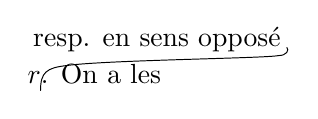
\begin{tikzpicture}[baseline=(orientation117.base)]
\node[anchor=base west,inner sep=0pt] (orientation117) at (0,0) {$r$. On a les};
\node[anchor=south west,inner sep=0pt] (respsens117)
  at ([xshift=2pt,yshift=4pt]orientation117.north west) {\inserted{resp. en sens opposé}};
\draw[line width=.35pt] (.17,-.09)
  .. controls (.17,.15) and (.25,.20) .. (.50,.23)
  .. controls (1.0,.30) and ([xshift=-6pt,yshift=-2pt]respsens117.south east)
  .. ([xshift=-1pt,yshift=-1pt]respsens117.south east)
  .. controls ([xshift=2pt,yshift=-1pt]respsens117.south east)
  and ([xshift=3pt,yshift=1pt]respsens117.south east)
  .. ([xshift=2pt,yshift=2pt]respsens117.south east);
\end{tikzpicture} relations

\figure{
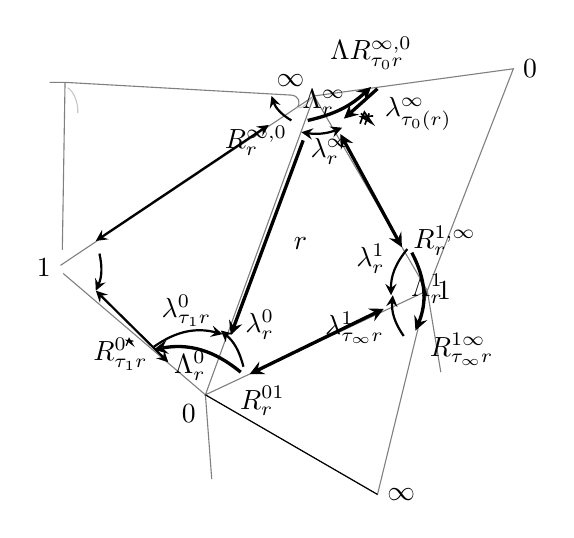
\begin{tikzpicture}[scale=1.15,>=stealth]
\coordinate (A) at (1.75,0.95);\coordinate (B) at (4.2,2.1);\coordinate (C) at (2.95,4.25);
\coordinate (D) at (0.15,2.35);\coordinate (E) at (5.15,4.55);\coordinate (F) at (3.65,-0.15);\coordinate (G) at (0.2,4.4);
% Pencil framework: separate tips at the outer 1 and literal local pen details.
\draw[gray] (C)--(E)--(B)--(F)--(A);
\draw[gray] (A)--(B)--(C)--cycle (A)--(1.82,0.02) (B)--(4.35,1.2);
\draw[gray] (G)--(.17,2.55);
\draw[gray] (.15,2.38)--(C);
\draw[gray] (.18,2.29)--(A);
\draw[gray] (G)--(.03,4.4);
\draw[gray!45,thin] (.23,4.34)
  .. controls (.29,4.31) and (.35,4.18) .. (.34,4.06);
% The faint intervening contour does not settle continuity at this junction.
\draw[gray] (G)--(2.70,4.26)
  .. controls (2.78,4.25) and (2.81,4.18) .. (2.76,4.12);
\draw[gray!45,thin] (2.76,4.12)
  .. controls (2.83,4.10) and (2.88,4.19) .. (C);
\draw[thin] (A)--(F);
\draw[very thick,->] (2.83,3.76)--(2.03,1.61);
\draw[very thick,<->] (2.24,1.18)--(3.72,1.9);
\draw[very thick,<->] (3.92,2.58)--(3.24,3.83);
\draw[thick,<->] (0.54,2.65)--(2.45,3.93);
\draw[thick,->] (0.58,2.51) to[bend left=18] (0.54,2.10);
\draw[thick,<->] (0.54,2.10)--(1.34,1.31);
\draw[thick,->] (2.17,1.26) to[bend right=18] (1.92,1.66);
\draw[thick,->] (1.18,1.48) to[bend left=25] (1.94,1.62);
\draw[very thick,->] (2.14,1.20) to[bend right=25] (1.18,1.45);
\draw[thick,->] (3.98,2.56) to[bend right=20] (3.80,2.05);
\node[inner sep=0pt,font=\tiny,rotate=-20] at (3.98,2.56) {$\unsure{\blacktriangle}$};
\draw[thick,->] (3.94,1.60) to[bend left=20] (3.82,2.05);
\draw[very thick,->] (4.03,2.52) to[bend left=25] (4.07,1.66);
\draw[thick,<->] (2.81,3.85) to[bend right=15] (3.26,3.90);
\draw[thick,->] (2.70,3.98) to[bend left=20] (2.48,4.25);
\draw[very thick,->] (2.88,3.98) to[bend right=15] (3.58,4.35);
\draw[very thick,->] (3.65,4.33)--(3.28,4.00);
\node[below left] at (A) {$0$};\node[right] at (B) {$1$};\node[above left] at (C) {$\infty$};
\node[left] at (D) {$1$};\node[right] at (E) {$0$};\node[right] at (F) {$\infty$};\node at (2.8,2.62) {$r$};
\node[below] at (2.38,1.15) {$R_r^{01}$};
\node[left] at (1.22,1.40) {$R_{\tau_1r}^{0\unsure{\tikz[x=.045cm,y=.045cm,baseline=-.4ex]{\draw[line width=.45pt] (0,0)--(.8,2)--(1.8,.3)--(.2,1.5)--(2,1.3);}}}$};
\node at (1.54,1.88) {$\lambda_{\tau_1r}^0$};\node at (1.58,1.27) {$\Lambda_r^0$};\node at (2.35,1.72) {$\lambda_r^0$};
\node[right] at (3.94,2.65) {$R_r^{1,\infty}$};\node[right] at (4.12,1.45) {$R_{\tau_\infty r}^{1\infty}$};
\node[left] at (3.84,2.45) {$\lambda_r^1$};\node[left] at (3.83,1.69) {$\lambda_{\tau_\infty r}^1$};\node at (4.20,2.12) {$\Lambda_r^1$};
\node[left] at (2.76,3.76) {$R_r^{\infty,0}$};\node[above] at (3.58,4.44) {$\deleted{\unsure{\Lambda}}R_{\tau_0r}^{\infty,0}$};
\node at (3.13,3.64) {$\lambda_r^\infty$};\node at (4.10,4.05) {$\lambda_{\tau_0(r)}^\infty$};\node at (3.06,4.18) {$\Lambda_r^\infty$};
\node[inner sep=0pt] at (3.53,3.98) {$\unsure{\tikz[x=.055cm,y=.055cm,baseline=-.5ex]{\draw[line width=.6pt] (0,0)--(1,2.7)--(2.8,.1)--(.3,1.6)--(3,1.8);\draw[line width=.6pt] (.2,2.4)--(2.5,.2) (1.1,-.2)--(2.1,2.4);}}$};
\end{tikzpicture}
}
\[
(14)\qquad 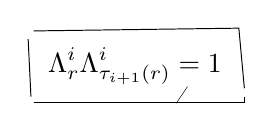
\begin{tikzpicture}[baseline=(eq14a.base)]
\node[inner sep=5pt] (eq14a) {$\displaystyle \Lambda_r^i\Lambda_{\tau_{i+1}(r)}^i=1$};
\draw[line width=.35pt] ([xshift=0pt,yshift=1pt]eq14a.north west)
  -- ([xshift=1pt,yshift=2pt]eq14a.north east)
  -- ([xshift=3pt,yshift=4pt]eq14a.south east);
\draw[line width=.35pt] ([xshift=-2pt,yshift=-2pt]eq14a.north west)
  -- ([xshift=-1pt,yshift=1pt]eq14a.south west);
\draw[line width=.35pt] ([xshift=0pt,yshift=-1pt]eq14a.south west)
  -- ([xshift=3pt,yshift=-1pt]eq14a.south east)
  -- ([xshift=3pt,yshift=1pt]eq14a.south east);
% Fine source trace; its origin and function remain uncertain.
\draw[line width=.18pt] ([xshift=15pt,yshift=-1.4pt]eq14a.south)
  -- ([xshift=19pt,yshift=4.6pt]eq14a.south);
\end{tikzpicture}\qquad
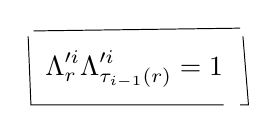
\begin{tikzpicture}[baseline=(eq14b.base)]
\node[inner sep=5pt] (eq14b) {$\displaystyle \Lambda_r^{\prime i}\Lambda_{\tau_{i-1}(r)}^{\prime i}=1$};
\draw[line width=.35pt] ([xshift=1pt,yshift=2pt]eq14b.north west)
  -- ([xshift=1pt,yshift=3pt]eq14b.north east);
\draw[line width=.35pt] ([xshift=-1pt,yshift=0pt]eq14b.north west)
  -- ([xshift=0pt,yshift=-1pt]eq14b.south west)
  -- ([xshift=-5pt,yshift=-1pt]eq14b.south east);
\draw[line width=.35pt] ([xshift=2pt,yshift=0pt]eq14b.north east)
  -- ([xshift=4pt,yshift=-1pt]eq14b.south east)
  -- ([xshift=1pt,yshift=-1pt]eq14b.south east);
\end{tikzpicture}
\]

\mspage{116}
